% RoadFix complete project report (15 November 2026): system, dataset, models, training, metrics, results,
% size and progress.  Compile: pdflatex main.tex  (run twice for the table of contents).
% Diagrams and charts are pre-rendered PDFs in figures/; their TikZ/pgfplots sources are in figures/src/.  See README.md.
\documentclass[11pt,a4paper]{article}

\usepackage[T1]{fontenc}
\usepackage[utf8]{inputenc}
\usepackage{lmodern}
\usepackage{microtype}
\usepackage[margin=2.2cm]{geometry}
\usepackage{amsmath,amssymb}
\usepackage{booktabs}
\usepackage{tabularx}
\usepackage{longtable}
\usepackage{array}
\usepackage{float}
\usepackage{graphicx}
\usepackage[table]{xcolor}
\usepackage{enumitem}
\usepackage{fancyhdr}
\usepackage{caption}
\usepackage[hidelinks]{hyperref}

\definecolor{gmblue}{HTML}{0B3D6E}
\definecolor{gmok}{HTML}{1E7B34}
\definecolor{gmwarn}{HTML}{B35C00}
\definecolor{gmbad}{HTML}{A32020}
\definecolor{gmgrey}{HTML}{5A5F66}
\definecolor{gmlight}{HTML}{EEF3F8}
\definecolor{gmteal}{HTML}{1B7A8C}

\newcommand{\done}{\textcolor{gmok}{\textbf{Done}}}
\newcommand{\partly}{\textcolor{gmwarn}{\textbf{Partly}}}
\newcommand{\pending}{\textcolor{gmbad}{\textbf{Pending}}}
\newcommand{\pass}{\textcolor{gmok}{\textbf{PASS}}}
\newcommand{\fail}{\textcolor{gmbad}{\textbf{FAIL}}}
\newcommand{\code}[1]{\texttt{\small #1}}
\newcommand{\INR}{INR~}

\setlist{itemsep=2pt,topsep=4pt}
\setlength{\parskip}{4pt}
\setlength{\parindent}{0pt}
\setlength{\emergencystretch}{3em}
\renewcommand{\arraystretch}{1.18}

\pagestyle{fancy}
\fancyhf{}
\lhead{\small RoadFix --- Potholes, Fixed for Good}
\rhead{\small Complete project report, 15 November 2026}
\cfoot{\small \thepage}
\setlength{\headheight}{14pt}



\begin{document}

% ================================================================================================ title
\begin{titlepage}
  \centering
  \vspace*{2.2cm}
  {\Huge\bfseries\color{gmblue} RoadFix\par}
  \vspace{4mm}
  {\Large Potholes, Fixed for Good\par}
  \vspace{10mm}
  {\large Bus-camera pothole detection $\rightarrow$ metric depth, area and volume with uncertainty
   $\rightarrow$ IRC:82 severity and priority $\rightarrow$ IRC:116 / SP:100 repair plan $\rightarrow$
   work orders, SLA escalation, bus-verified repair and defect-liability tracking\par}
  \vspace{14mm}
  {\Large\bfseries Complete project report\par}
  \vspace{3mm}
  {\large How the system works, the dataset, the models, the training run, the metrics, \\
   the size of the project, and the progress so far\par}
  \vspace{12mm}
  {\large Telangana R\&B / Municipal Administration challenge\par}
  \vspace{4mm}
  {\large Status as of 15 November 2026\par}
  \vfill
  \begin{minipage}{0.88\textwidth}\small
  \textbf{How to read this report.} Section~\ref{sec:summary} gives the whole status on one page.
  Sections~\ref{sec:problem}--\ref{sec:steps} explain what the system does and how a pothole travels through it.
  Sections~\ref{sec:dataset}--\ref{sec:results} are the machine-learning part: the dataset, the models, the training
  run, what each metric means, and the results. Sections~\ref{sec:measure}--\ref{sec:size} cover measurement
  accuracy, the end-to-end demo and the size of the project. Sections~\ref{sec:status}--\ref{sec:run} list progress,
  pending work and how to run everything.

  \textbf{Every number is copied from the project's own artefacts} (\code{reports/model\_eval.json},
  \code{runs/seg/y26n\_seg\_india\_laptop/}, \code{data/datasets/india\_pothole\_seg4/stats.json},
  \code{reports/REPORT.md}, \code{reports/demo\_summary.json}, \code{docs/DECISIONS.md}). Time and cost figures for
  the future are \emph{estimates} and are labelled as such.
  \end{minipage}
\end{titlepage}

\tableofcontents
\newpage

% ================================================================================================ 1
\section{Status at a glance}\label{sec:summary}

\textbf{The software is complete and verified on the development laptop.} All thirteen work packages (WP0--WP12)
are implemented and tested: measurement, geo services, database and API, processing workers, operations (work
orders, SLA, verification, DLP), web app, bus simulator, validation scripts, documentation and a one-command demo.

\textbf{The first trained detector exists, but it is not good enough yet.} On 14--15 November 2026 a small
segmentation model (YOLO26n-seg, 3.1 million parameters) was trained for 20 epochs on the laptop's 2\,GB GPU. It is
\textbf{2.5$\times$ better} than the starter model (pothole box mAP50 0.221 vs 0.0885) and is the first model that
draws pothole outlines, but it is far below the acceptance target of 0.70. It is now the working detector of the
system as a stopgap.

\begin{center}
\begin{tabularx}{\textwidth}{@{}l X r@{}}
\toprule
\textbf{Check} & \textbf{What it shows} & \textbf{Result}\\
\midrule
Python test suite & 276 automated tests (unit, API, workers, geo, end-to-end) & \textcolor{gmok}{276 passed}\\
Web application & unit tests, production build, offline smoke checks, browser tests & \textcolor{gmok}{38 / OK / 15 / 3}\\
Measurement geometry & 16 synthetic road scenes with exact truth & \textcolor{gmok}{16/16, vol.\ err.\ $\le$ 2.9\,\%}\\
Uncertainty ($\sigma$) & 200 noisy trials, truth inside $\pm2\sigma$ & \textcolor{gmok}{coverage 1.00 ($\ge$ 0.90)}\\
Full demo & 3 simulated buses, 3 routes, 2 days, real Hyderabad roads & \textcolor{gmok}{4/4 checks, 732\,s}\\
Detector, boxes & pothole box mAP50 on RDD-India test (target $\ge$ 0.70) & \textcolor{gmbad}{0.221 (was 0.0885)}\\
Detector, masks & mean mask IoU of found potholes (target $\ge$ 0.65) & \textcolor{gmwarn}{0.689 (only 149 found)}\\
Real-camera depth & staged foam-board targets with a calibrated camera & \textcolor{gmbad}{not done yet}\\
\bottomrule
\end{tabularx}
\end{center}

\textbf{In one sentence:} the whole loop from camera to verified repair works and is tested, measurement geometry is
proven on exact synthetic data, and the two things that decide real-world accuracy --- a strong detector and a
real-camera depth check --- are the next steps.

\textbf{Estimated time to a validated pilot} (one to two developers; estimate, not a commitment): about
\textbf{1--2 weeks} for a target-grade model on an RTX-class GPU, \textbf{3--4 months} until the system is ready for
real buses, and about \textbf{6 months} including a 12-week pilot through a monsoon (Section~\ref{sec:pending}).

% ================================================================================================ 2
\section{The problem and the idea}\label{sec:problem}

Potholes on city roads are reported late, measured by eye, repaired without proof, and often come back within
months. Four gaps cause most of this:
\begin{enumerate}
  \item \textbf{Finding them.} Surveys are occasional and manual; complaints arrive after the damage.
  \item \textbf{Measuring them.} Material and money are estimated by eye (``a few bags''), so neither the plan nor the
        bill can be checked.
  \item \textbf{Proving the repair.} A contractor's ``done'' photo is the only evidence that a repair happened and
        lasted.
  \item \textbf{Accountability.} When a repaired pothole reappears inside the contractor's defect-liability period
        (DLP), nobody notices in time to claim a free rework.
\end{enumerate}

\textbf{The idea.} TGSRTC buses already drive every arterial road many times a day. A camera behind the windscreen
turns every trip into a free survey. RoadFix closes the loop:
\emph{find $\rightarrow$ measure $\rightarrow$ prioritise $\rightarrow$ plan $\rightarrow$ repair $\rightarrow$ prove
the repair with later bus passes $\rightarrow$ catch the comeback}. It follows Indian standards throughout
(IRC:82-2015 for severity, IRC:116-2014 and IRC:SP:100-2014 for cold-mix repair) and is built for Indian roads.

Three rules run through the whole system:
\begin{itemize}
  \item every measurement carries an uncertainty $\sigma$, the method used, and a quality score;
  \item cold-mix bags are always given as a low--high range, never as an ``exact'' number;
  \item demo calibrations are marked \code{certified=false} and are never used for billing.
\end{itemize}

% ================================================================================================ 3
\section{System architecture}\label{sec:arch}

\begin{figure}[H]
\centering
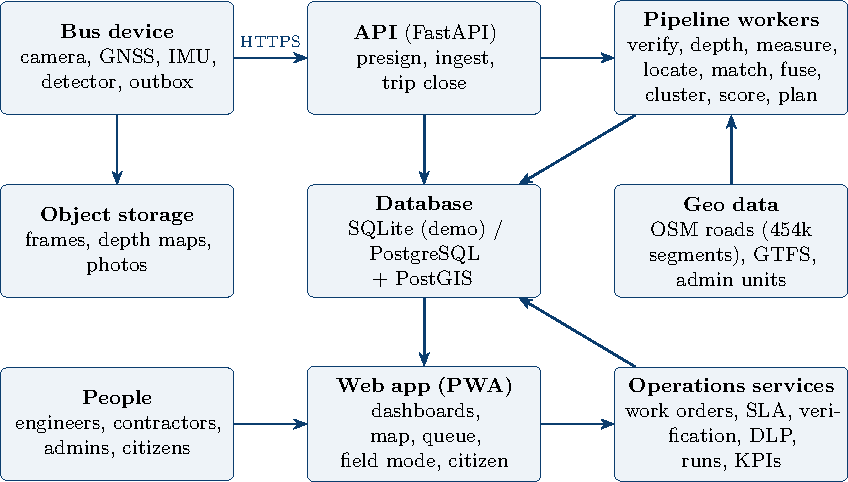
\includegraphics{figures/fig-01-architecture.pdf}
\caption{Main components. In the demo everything runs on one laptop (SQLite, filesystem storage, pipeline inside the
API process); production uses PostgreSQL/PostGIS, S3-compatible storage and separate worker processes.}
\end{figure}

\begin{center}
\begin{tabularx}{\textwidth}{@{}>{\raggedright\arraybackslash}p{36mm} X@{}}
\toprule
\textbf{Folder} & \textbf{Role}\\
\midrule
\code{edge/} & bus side: simulator (\code{sim/}), wire protocol (\code{protocol.md}, \code{schema/}), Jetson runner, Android skeleton\\
\code{measure/} & depth backends, road-plane fit, cavity measurement, uncertainty, fusion, IRC severity\\
\code{geo/} & ground-point location, map-matching, clustering, bus-pass counting, jurisdiction\\
\code{priority/}, \code{repair/} & priority score and SLA hours; repair planner (bags, materials, labour, cost)\\
\code{server/} & API, database models, workers (pipeline stages, ops ticks), operations services\\
\code{ml/} & segmenter interface, training, evaluation, export, pseudo-labelling\\
\code{data/} & dataset download, build and derivation scripts; fixed splits\\
\code{web/} & React progressive web app (Telugu first, also Hindi and English), offline field mode\\
\code{gis/} & map layers (zones, circles, wards, CRMP packages)\\
\code{scripts/}, \code{docs/}, \code{reports/} & demo and validation scripts; method and operations documents; results\\
\bottomrule
\end{tabularx}
\end{center}

% ================================================================================================ 4
\section{How the system works, step by step}\label{sec:steps}

This section follows one pothole from the camera to the closed, verified repair.

\begin{figure}[H]
\centering
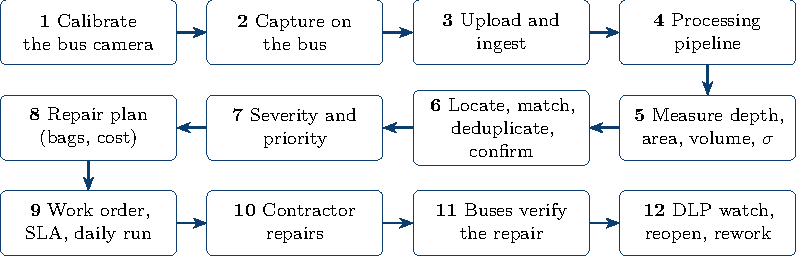
\includegraphics{figures/fig-02-thirteen-steps.pdf}
\caption{The twelve steps. Step 13 (dashboards, citizens, public reporting) reads from all of them.}
\label{fig:flow}
\end{figure}

\subsection{Step 1 --- Calibrate the bus camera}
Depth from a single camera is only metric if the system knows the camera's geometry. Each device gets a
\emph{calibration certificate} (\code{configs/cameras/*.json}):
\begin{itemize}
  \item \textbf{Intrinsics} (once per camera model): focal lengths $f_x, f_y$, principal point $c_x, c_y$ and lens
        distortion, from 20--25 photos of a $9\times6$ checkerboard; accepted below 0.3 pixels reprojection error.
  \item \textbf{Extrinsics} (every bus, about 10 minutes at the depot): camera height $h_{\text{true}}$ measured with a
        tape ($\pm1$\,cm; about 2.2--2.5\,m on a bus), pitch, roll and yaw from four cones at 3/5/8/12\,m; accepted if
        a painted $1\times1$\,m square at 5\,m is reconstructed within 5\,\%.
  \item \textbf{Drift checks} on every trip: if the camera height implied by the road plane drifts by more than 5\,\%
        or the pitch by more than $3^\circ$, the server raises an alert and the bus is recalibrated.
\end{itemize}
A certificate becomes \code{certified=true} only when both acceptance tests pass, and billing-grade only after a
per-device truth fit on at least 20 inspector-measured potholes (\code{docs/CALIBRATION\_SOP.md}, Telugu and English).

\subsection{Step 2 --- Capture on the bus}
The device (an Android phone, a Jetson box, or the simulator) runs the same loop: a \textbf{keyframe} every 4\,m of
travel above 5\,km/h; \textbf{detection} by the on-device segmenter (class, confidence, box, outline polygon, track
id; at most 3 keyframes per tracked pothole); \textbf{privacy blur} of faces and number plates on the device; one
JSON \textbf{observation} per keyframe (device, trip, time, GNSS fix, IMU summary, frame key, a fixed
\code{client\_uuid} so resending is harmless); IMU \textbf{jolts} that confirm a pothole exists but never set its
depth; \textbf{trip fixes} every second with a \code{cam\_active} flag (later used to prove clean passes); and a
durable \textbf{outbox} that keeps everything until the server acknowledges it.

\subsection{Step 3 --- Upload and ingest}
Over LTE or depot Wi-Fi, in a fixed order (\code{edge/protocol.md}): \code{POST /v1/edge/presign} and \code{PUT} of
frames; \code{POST /v1/ingest/observations} (up to 200 per batch, idempotent); \code{POST /v1/ingest/trip-fixes}
(up to 600 per batch); \code{POST /v1/ingest/trip-close}, which builds the trip geometry and runs bus-pass counting
and repair verification. Every call can be retried safely; the server removes duplicates.

\subsection{Step 4 --- The processing pipeline}
Each observation runs through nine stages:
\begin{center}

\includegraphics{figures/fig-03-pipeline.pdf}
\end{center}
\textbf{verify}: a second detector checks each detection. \textbf{depth}: a metric depth model estimates the distance
of every pixel. \textbf{measure}: depth, area and volume with $\sigma$. \textbf{locate}/\textbf{match}: ground
position and road segment. \textbf{fuse}: frames are combined into one measurement per pass. \textbf{cluster}: the
observation joins an existing pothole or creates a new one. \textbf{score}: severity and priority. \textbf{plan}:
repair plan. A failing stage is recorded as an error; no stage quietly falls back to a cruder method.

\subsection{Step 5 --- Measure depth, area and volume (with \texorpdfstring{$\sigma$}{sigma})}
Details: \code{docs/DEPTH\_METHOD.md}.
\begin{enumerate}
  \item \textbf{Back-projection.} For pixel $(u,v)$ with depth $Z$: $X=(u-c_x)Z/f_x$, $Y=(v-c_y)Z/f_y$.
  \item \textbf{Road plane.} RANSAC fits a plane $n\cdot p + d = 0$ to road pixels (lower 65\,\% of the image,
        potholes masked out, 2.5--14\,m, 15\,mm inlier band). The frame is rejected if fewer than half the points fit,
        the residual exceeds 25\,mm, or the pitch differs from the calibration by more than $4^\circ$.
  \item \textbf{Scale lock.} $\hat h=|d|$ is the camera height the depth model believes in; multiplying every depth by
        $s=h_{\text{true}}/\hat h$ (allowed 0.5--2.0) removes the 5--30\,\% absolute-scale error of monocular depth
        models with one tape measurement.
  \item \textbf{Local road surface.} Around each pothole (ring 0.3--1.2\,m) a quadratic surface
        $y_s=a+bx+cz+dx^2+ez^2+fxz$ follows camber and ruts.
  \item \textbf{Cavity.} Per mask pixel: depth below road $\delta_i=\max(0,\,y_s(x_i,z_i)-y_i)$, ground footprint
        $a_i=(Z_i/f_x)(Z_i/f_y)/\cos\theta_i$.
  \item \textbf{Metrics.} $A=\sum_i a_i$, $V=\sum_i \delta_i a_i$, $d_{p95}$ = area-weighted 95th percentile of
        $\delta_i$ (the design depth), plus length and width from the minimum-area rectangle.
  \item \textbf{Uncertainty.} $\sigma_{Z,i}=k Z_i^2$ with $k=4\times10^{-4}\,\text{m}^{-1}$ until a per-device fit
        exists, combined with the surface-fit residual and the scale uncertainty into $\sigma$ for $d_{p95}$, $A$, $V$.
  \item \textbf{Quality} $q\in[0,1]$: product of gates for range (best 3--7\,m, zero beyond 12\,m), blur, light, mask
        confidence, plane fit and mask size.
  \item \textbf{Fusion.} Frames with $q<0.2$ or beyond $3\sigma$ are dropped; the rest are averaged with weights
        $q_j/\sigma_j^2$, first per pass, then per pothole.
  \item \textbf{Water.} A water-filled pothole gets \emph{unknown} depth (never the water surface), a severity lower
        bound from its width, and a re-measure 48\,h after rain.
\end{enumerate}

\subsection{Step 6 --- Locate, match to a road, deduplicate, confirm}
\begin{itemize}
  \item \textbf{Ground point}: GNSS fix advanced by receiver latency and offset by the measured forward and lateral
        distance; $\sigma_{\text{pos}}=\sqrt{\text{gps\_accuracy}^2+(0.05D)^2}$.
  \item \textbf{Map-matching}: nearest OpenStreetMap segment within 25\,m whose direction agrees with the bus heading
        ($\pm45^\circ$) $\rightarrow$ road, direction, chainage, lane band.
  \item \textbf{Clustering}: same road and direction within about 6\,m (or $2.5\sigma$) = same pothole.
  \item \textbf{Confirmation}: \code{candidate} $\rightarrow$ \code{confirmed} after $\ge2$ passes from $\ge2$ trips,
        or one pass plus a citizen report within 25\,m, or one pass plus an IMU jolt with quality $\ge0.6$.
  \item \textbf{Owner}: the road gives the agency and CRMP contract; unknown owners go to a \emph{jurisdiction queue}.
\end{itemize}

\subsection{Step 7 --- Severity and priority}
\textbf{Severity (IRC:82-2015):} small ($d_{p95}\le25$\,mm and width $\le200$\,mm), medium ($\le50$\,mm and
$\le500$\,mm), otherwise large. \textbf{Priority} (0--100, editable per agency, versioned):
\[ P = 100\cdot\operatorname{clip}\big(0.30\,S+0.25\,E+0.20\,V+0.15\,T+0.10\,M,\ 0,\ 1\big) \]
with $S$ severity (plus wheel-path, junction, jolt bonuses), $E$ exposure (road class, bus passes per day), $V$
vulnerability (schools, hospitals, bus stops, markets within 200\,m, unlit roads), $T$ age against the SLA and
complaints, $M$ monsoon factors (season, recent rain, waterlogging hotspot).

\subsection{Step 8 --- Repair plan}
Following IRC:82, IRC:116-2014 and IRC:SP:100-2014: square cut with 0.125\,m margin, $A_{\text{cut}}=(L+0.25)(W+0.25)$;
design depth $\max(d_{p95},50\,\text{mm})$ rounded up to 5\,mm (two layers above 75\,mm); mix mass
$M=A_{\text{cut}}\cdot d\cdot\rho\cdot(1+w)$ with $\rho=2200$\,kg/m$^3$ and 12\,\% wastage; bags
$=\lceil M/25\,\text{kg}\rceil$ with a low--high range from $\sigma_M$; then emulsion, sand, labour and cost from the
rate card. \textbf{Worked example} (a unit test): $0.50\times0.40$\,m, $d_{p95}=60$\,mm $\rightarrow$ cut
$0.4875$\,m$^2$, 72.1\,kg of mix, \textbf{3 bags (range 3--4)}, about \INR1,406 against a reported baseline of
\INR7,396 per pothole.

\subsection{Step 9 --- Work order, SLA and the daily repair run}
A work order for one or more potholes goes to the contractor of the road's CRMP package. The SLA clock starts at issue
(24\,h arterial; 72\,h other roads in monsoon; 168\,h off-season or R\&B). \textbf{Escalation} (checked every 5
minutes): 50\,\% of SLA $\rightarrow$ AE; breach $\rightarrow$ DEE; +24\,h $\rightarrow$ EE; +72\,h $\rightarrow$
Zonal Commissioner. \textbf{Daily run} (06:00 IST per circle): nearest-neighbour route capped by crew hours, printed
as an \emph{indent} (bags, emulsion, sand, crew hours, cost).

\subsection{Step 10 --- The contractor repairs}
Field mode of the web app (works offline): \code{acknowledged} $\rightarrow$ \emph{before} photo $\rightarrow$
\code{in\_progress} (bag lot) $\rightarrow$ \emph{after} photo and bags used $\rightarrow$ \code{repaired\_claimed}.
A contractor acts only on their own work orders and can never verify their own repair; every transition is audited.

\subsection{Step 11 --- Buses verify the repair}
A claim is not a repair. Each later bus pass over the spot (same road, direction, lane band, camera on) without a
detection is a \emph{clean pass}. The work order becomes \code{verified\_closed} after \textbf{$\ge3$ clean passes from
$\ge2$ trips within 14 days} (plus a 10\,\% engineer QC sample). Only verified work is eligible for invoicing.

\subsection{Step 12 --- DLP watch, reopen and rework}
If a bus detects the pothole again inside the defect-liability period (6 months for a patch; 5 years for a CRMP
package), it is \code{reopened}, a \code{dlp\_event} with an evidence package is recorded, and a zero-pay rework work
order is drafted for the same contractor --- evidence for the engineer, not an automatic penalty.

\begin{figure}[H]
\centering
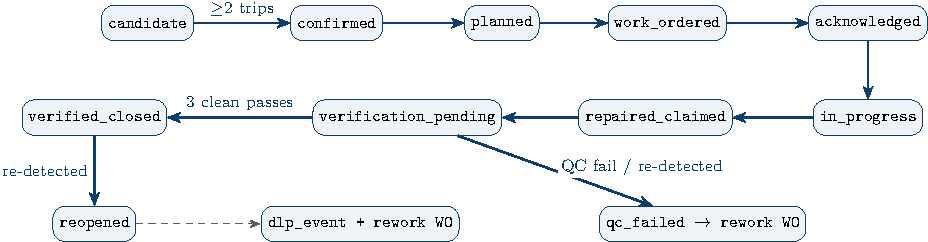
\includegraphics{figures/fig-04-pothole-states.pdf}
\caption{Pothole life cycle (simplified; \code{rejected}, \code{archived} and \code{recurrence\_watch} omitted).}
\end{figure}

\subsection{Step 13 --- Dashboards, citizens and public reporting}
The web app (Telugu first, also Hindi and English) offers a zonal KPI dashboard, a severity/priority map, a pothole
page (frames, mask, depth cross-section, measurement $\pm\sigma$, repair plan), the priority queue, work orders,
repair runs and indents, the offline field mode, contractor scorecards, an admin area (weights, rate card, SLA, admin
units, jurisdiction queue, audit log), a citizen page to report and track a pothole, and a public ward league.

% ================================================================================================ 5
\section{The dataset}\label{sec:dataset}

The detector has to learn what a pothole looks like \emph{on Indian roads}, from a bus or car camera, and has to draw
its outline (a mask), because the outline is what the measurement step integrates over. This section explains where
the training images come from, how they were turned into one dataset, and how big it is.

\subsection{Sources}
\begin{center}
\small
\begin{tabularx}{\textwidth}{@{}>{\raggedright\arraybackslash}p{37mm} >{\raggedright\arraybackslash}p{26mm} X >{\raggedright\arraybackslash}p{24mm}@{}}
\toprule
\textbf{Source} & \textbf{Labels} & \textbf{Use in RoadFix} & \textbf{Licence}\\
\midrule
RDD2022 --- India part (CRDDC 2022) & boxes for road damage (D00, D10, D20, D40) & main source of Indian potholes and cracks; \textbf{the test split is drawn from it}; 720$\times$720 frames & CC BY-SA 4.0\\
RDD2022 --- other countries (Japan, Czech Rep., USA, China) & boxes & only frames that contain potholes (D40), \textbf{train split only}; 600$\times$600 frames & CC BY-SA 4.0\\
eYantra ``Semantic Segmentation Datasets of Indian Roads'' (IIT Bombay) & pixel polygons & the only Indian set with real \emph{masks}; gives manholes / drain covers; 1280$\times$720 frames & GPL-2.0 (prototype only)\\
BharatPotHole & boxes & simulator frames only; \textbf{excluded from training} (licence unverified) & unverified\\
\bottomrule
\end{tabularx}
\end{center}
Licences matter because the system is meant for government deployment: \code{docs/LICENCES.md} records each one and
the open decisions (for example, GPL-2.0 eYantra data must not end up in a deployed model without a decision).

\subsection{Classes}
The system has a fixed 7-class vocabulary (\code{configs/classes.yaml}, part of the frozen bus protocol): pothole,
pothole\_water, alligator\_crack, crack, manhole, speed\_breaker, utility\_cut. Three of these have \textbf{no labelled
examples} in any usable source, so the training dataset \code{india\_pothole\_seg4} keeps only the four classes that
do (decision D15). The vocabulary itself is unchanged, so a future model with water or speed-breaker data plugs in
without a protocol change.

\begin{center}
\small
\begin{tabularx}{\textwidth}{@{}c l X@{}}
\toprule
\textbf{Id} & \textbf{Class} & \textbf{Where the examples come from}\\
\midrule
0 & pothole & RDD2022 \code{D40}\\
1 & alligator\_crack & RDD2022 \code{D20}\\
2 & crack & RDD2022 \code{D00} (longitudinal) and \code{D10} (transverse), merged\\
3 & manhole & eYantra ``shallow'' polygons, which on inspection are manhole and drain covers (decision D13). The class
exists to absorb these look-alikes so they are not reported as potholes.\\
\bottomrule
\end{tabularx}
\end{center}
Water-filled potholes are handled by the measurement step (unknown depth, re-measure after rain), not by the
detector.

\subsection{How the dataset is built}
\begin{figure}[H]
\centering
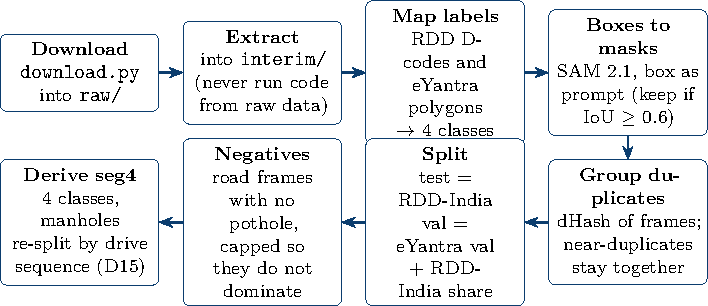
\includegraphics{figures/fig-05-dataset-build.pdf}
\caption{Dataset pipeline: \code{data/build\_dataset.py} builds \code{india\_pothole\_seg}; \code{data/derive\_dataset.py}
derives the 4-class \code{india\_pothole\_seg4} from it with hard links (the build is never modified).}
\end{figure}

Four details matter for understanding the results:
\begin{itemize}
  \item \textbf{Masks from boxes.} RDD2022 has only boxes. Each box is given to SAM 2.1 (a general ``segment
        anything'' model) as a prompt; the resulting mask is kept if its bounding box agrees with the original box
        (IoU $\ge$ 0.6), otherwise the box itself is used as the outline. These are \emph{pseudo-masks}: good, but not
        hand-drawn. Only eYantra has hand-drawn masks.
  \item \textbf{No leakage between splits.} Consecutive frames of one drive look almost the same. Frames are grouped by
        a perceptual hash and a whole group always goes into one split, so the test set never contains a near-copy of
        a training image.
  \item \textbf{Manholes re-split by drive sequence.} All manholes come from only six eYantra drive sequences. Whole
        sequences were assigned to splits; every possible assignment was tried and the one closest to 70/15/15 was
        kept. The best possible is 90/5/5 (train 1,269, val 76, test 69 instances).
  \item \textbf{Image format.} YOLO segmentation format: one \code{.jpg} and one \code{.txt} per image; each line is a
        class id followed by the polygon's corner points, normalised to 0--1.
\end{itemize}

\subsection{Size of the dataset}
\begin{center}
\begin{tabular}{@{}l r r r r r r r@{}}
\toprule
\textbf{Split} & \textbf{Images} & \textbf{with labels} & \textbf{pothole} & \textbf{alligator} & \textbf{crack} & \textbf{manhole} & \textbf{instances}\\
\midrule
train & 4,465 & 4,032 & 3,926 & 2,431 & 1,995 & 1,269 & 9,621\\
val   &   933 &   297 &   174 &   156 &   118 &    76 &   524\\
test  & 1,018 &   565 & 1,038 &   215 &   177 &    69 & 1,499\\
\midrule
\textbf{total} & \textbf{6,416} & \textbf{4,894} & \textbf{5,138} & \textbf{2,802} & \textbf{2,290} & \textbf{1,414} & \textbf{11,644}\\
\bottomrule
\end{tabular}
\end{center}

\begin{center}
\begin{tabular}{@{}l r r r l@{}}
\toprule
\textbf{Images by source} & \textbf{train} & \textbf{val} & \textbf{test} & \textbf{resolution}\\
\midrule
RDD2022 India (\code{rddin\_*}) & 2,418 & 600 & 514 & 720 $\times$ 720\\
RDD2022 other countries, pothole frames (\code{rddfx\_*}) & 1,593 & --- & --- & 600 $\times$ 600\\
eYantra Indian roads (\code{ey\_*}) & 454 & 333 & 504 & 1280 $\times$ 720\\
\bottomrule
\end{tabular}
\end{center}

\begin{figure}[H]
\centering
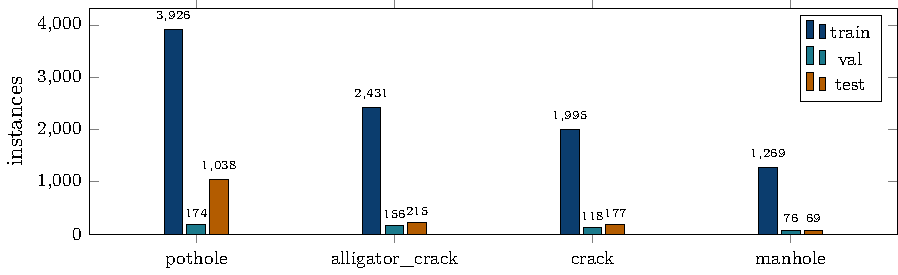
\includegraphics{figures/fig-06-instances-per-class.pdf}
\caption{Labelled instances per class and split.}
\end{figure}

\textbf{On disk:} original downloads 13\,GB (\code{data/raw}), extracted sources plus the SAM 2.1 mask cache and geo
data 3.4\,GB (\code{data/interim}), both built datasets together 788\,MB (\code{data/datasets}; images are hard
links, so the 6,416 images are stored once).

\subsection{Known weaknesses of the dataset}
These are not hidden; they explain a good part of the results in Section~\ref{sec:results}.
\begin{enumerate}
  \item \textbf{The validation set is small.} Only 297 of its 933 images contain any label, with just 174 potholes.
        Validation scores therefore jump by several points from one epoch to the next, and picking the ``best''
        epoch on it is partly luck.
  \item \textbf{36\,\% of training images are not Indian} (the 1,593 \code{rddfx} frames). They add pothole examples
        but from different roads, cameras and light.
  \item \textbf{Most masks are pseudo-masks}, and the original RDD boxes are loose and not always consistent, so the
        model learns from (and is scored against) imperfect outlines.
  \item \textbf{Manholes are only 5\,\% of val and test}, from a few drive sequences, so manhole scores are very noisy.
  \item \textbf{The test set is pothole-heavy} (1,038 potholes in 514 RDD-India frames), which suits the acceptance
        test but gives only 69--215 examples for the other classes.
\end{enumerate}

% ================================================================================================ 6
\section{The models}\label{sec:models}

RoadFix uses several neural networks, each for one job. Only the \emph{segmenter} is trained by the project; the
others are used as published.

\begin{center}
\small
\begin{tabularx}{\textwidth}{@{}>{\raggedright\arraybackslash}p{37mm} >{\raggedright\arraybackslash}X r r r@{}}
\toprule
\textbf{Model} & \textbf{Job in the system} & \textbf{Params} & \textbf{GFLOPs} & \textbf{File}\\
\midrule
\textbf{YOLO26n-seg, trained here} (\code{best.pt}) & \textbf{segmenter}: finds potholes, cracks, manholes and draws their outlines; \textbf{active now} (\code{SEG\_WEIGHTS}) & 3.08\,M & 10.4 & 6.6\,MB\\
YOLO26n-seg (COCO, Ultralytics) & starting point of the training above & 3.13\,M & --- & 6.7\,MB\\
YOLO26s-seg (COCO, Ultralytics) & starting point for the planned RTX 5080 training & 11.5\,M & 37.7 & 23.5\,MB\\
Bootstrap pothole YOLO26m (public) & day-0 detector until a model was trained; boxes only, 1 class & 21.8\,M & 75.0 & 44.0\,MB\\
Verifier YOLOv8s RDD (public) & second opinion on each detection; boxes only, 5 RDD classes & 11.1\,M & 28.7 & 67.1\,MB\\
Depth-Anything-V2 Metric Outdoor Base & metric depth per pixel (ViT-B encoder + DPT head) & 97.5\,M & --- & 372\,MB\\
SAM 2.1 hiera-small & \emph{offline only}: turns dataset boxes into masks & 46.1\,M & --- & 176\,MB\\
SegFormer-B0 (Cityscapes) & optional: marks non-road pixels before the road-plane fit & 3.7\,M & --- & 29\,MB\\
\bottomrule
\end{tabularx}
\end{center}
GFLOPs are for one 640$\times$640 image. Parameter counts of the Hugging Face models are from their weight files.

\subsection{How the segmenter works (YOLO26n-seg)}
\begin{figure}[H]
\centering
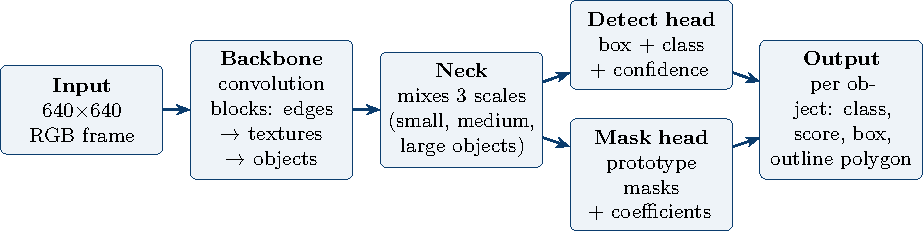
\includegraphics{figures/fig-07-segmenter.pdf}
\caption{The segmenter. Each detected object's mask is a weighted mix of a small set of shared ``prototype'' masks,
cropped to its box; this is what makes instance masks cheap enough for a phone or a Jetson.}
\end{figure}

\begin{itemize}
  \item \textbf{Why this model.} The ``n'' (nano) size is the largest that trains on the laptop's 2\,GB GPU and is the
        size that runs on a bus device (Android phone or Jetson). It has 3.08 million parameters and needs 10.4 billion
        operations per frame; the trained file is 6.6\,MB. On the laptop GPU it takes about 118\,ms per image
        including pre- and post-processing, against 175\,ms for the bigger bootstrap model.
  \item \textbf{Transfer learning.} It starts from weights trained on COCO (everyday objects) and is re-trained on the
        road dataset: the early layers already know edges and textures; the last layers learn the four road classes.
  \item \textbf{What it outputs.} For every object: class, confidence (0--1), box and outline polygon. The outline goes
        into the measurement step (Step 5), the class and confidence into the verify stage and the pothole record.
  \item \textbf{Model choice is a licence question too}: Ultralytics YOLO is AGPL-3.0 (\code{docs/LICENCES.md} \S4
        lists the options: Enterprise licence, publish the source, or switch to RF-DETR).
\end{itemize}

\subsection{How the depth model is used}
Depth-Anything-V2 Metric Outdoor estimates, for every pixel, the distance from the camera in metres. On its own its
absolute scale can be off by 5--30\,\%; RoadFix corrects this with the measured camera height (scale lock, Step 5).
It is the heaviest model (97.5\,M parameters) and runs on the server, not on the bus. On the laptop it takes
5--20\,s per frame on the CPU, so the demo uses a synthetic depth render instead and is labelled as such.

% ================================================================================================ 7
\section{Training the segmenter}\label{sec:training}

\subsection{Set-up}
\begin{center}
\small
\begin{tabularx}{\textwidth}{@{}>{\raggedright\arraybackslash}p{42mm} X@{}}
\toprule
\textbf{Item} & \textbf{Value}\\
\midrule
Run name, profile & \code{y26n\_seg\_india\_laptop}, profile \code{laptop\_mx330\_max} in \code{configs/model/}\\
Hardware & laptop: Intel i7-10510U, 15.8\,GB RAM, NVIDIA GeForce MX330 with 2\,GB (compute capability 6.1)\\
Software & Python 3.11, PyTorch 2.11 + CUDA 12.6, Ultralytics; Windows 11\\
Start weights & \code{weights/yolo26n-seg.pt} (COCO pre-trained)\\
Data & \code{india\_pothole\_seg4}: 4,465 train images (all used), 933 validation images\\
Image size, batch & 640$\times$640; batch 3 (chosen automatically to fill 90\,\% of GPU memory); 1,489 steps per epoch\\
Precision & 32-bit (half precision is not reliable on this GPU generation)\\
Epochs & planned 30, reduced to \textbf{20} after epoch 9 to finish in time; early stop after 10 epochs without improvement (not triggered)\\
Augmentation & mosaic (4 images in one) switched off for the last 5 epochs, brightness $\pm$50\,\%, rotation $\pm3^\circ$, left--right flip 50\,\%, scale $\pm$40\,\%\\
Other & images cached in RAM, 4 data-loader workers, fixed random seed 20261113, a checkpoint after every epoch\\
\bottomrule
\end{tabularx}
\end{center}

\subsection{Timeline}
\begin{center}
\small
\begin{tabular}{@{}l l l r@{}}
\toprule
\textbf{Session} & \textbf{Start (IST)} & \textbf{End (IST)} & \textbf{Epochs, wall time}\\
\midrule
1 & 14 Nov, 14:05 & 14 Nov, 20:57 (paused) & 1--9, 6.9\,h\\
2 (resumed from epoch 9) & 15 Nov, 13:36 & 15 Nov, 16:27 (finished) & 10--20, 2.8\,h\\
Evaluation on the test split & 15 Nov, 18:37 & 15 Nov, 18:40 & about 3\,min\\
\bottomrule
\end{tabular}
\end{center}
Total compute: 9.1\,h of training plus 0.6\,h of validation. In the second session an epoch took about
\textbf{12 minutes} (0.47\,s per step, GPU 67--74\,\% busy, at most 74\,$^\circ$C, 1.3--1.4 of 2.0\,GB GPU memory). The
first session's epochs took 23--71 minutes, and epoch 19 took 32 minutes; the training monitor flagged these as slow
epochs, the cause (other load on the laptop) was not recorded.

\subsection{Training curves}
\begin{figure}[H]
\centering
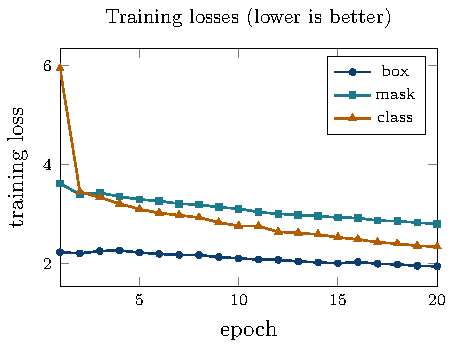
\includegraphics{figures/fig-08-training-losses.pdf}\hfill
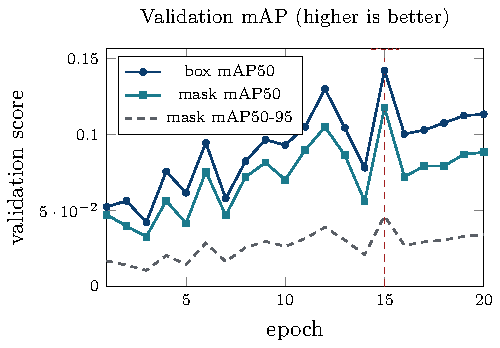
\includegraphics{figures/fig-09-validation-map.pdf}
\caption{Left: the model is still learning --- all three training losses fall steadily up to epoch 20. Right: the
validation score rises from 0.05 to about 0.11 but jumps around (small validation set); epoch 15 scored highest and
was saved as \code{best.pt}.}
\end{figure}

\begin{center}
\scriptsize\setlength{\tabcolsep}{4pt}
\begin{tabular}{cccccccccc}
\toprule
\textbf{Epoch} & \textbf{Min.} & \textbf{Box P} & \textbf{Box R} & \textbf{Box mAP50} & \textbf{Mask mAP50} & \textbf{Mask 50-95} & \textbf{Loss box} & \textbf{Loss mask} & \textbf{Loss class}\\
\midrule
1 & 26.9 & 0.336 & 0.092 & 0.052 & 0.047 & 0.017 & 2.24 & 3.62 & 5.93\\
2 & 25.2 & 0.334 & 0.143 & 0.056 & 0.040 & 0.014 & 2.21 & 3.40 & 3.46\\
3 & 31.4 & 0.076 & 0.134 & 0.042 & 0.033 & 0.010 & 2.26 & 3.43 & 3.34\\
4 & 76.2 & 0.330 & 0.118 & 0.075 & 0.056 & 0.020 & 2.27 & 3.36 & 3.21\\
5 & 64.7 & 0.113 & 0.187 & 0.061 & 0.041 & 0.014 & 2.23 & 3.30 & 3.10\\
6 & 37.7 & 0.167 & 0.189 & 0.094 & 0.075 & 0.028 & 2.20 & 3.27 & 3.03\\
7 & 34.5 & 0.219 & 0.136 & 0.058 & 0.047 & 0.016 & 2.18 & 3.21 & 2.98\\
8 & 44.6 & 0.164 & 0.150 & 0.082 & 0.072 & 0.025 & 2.18 & 3.20 & 2.93\\
9 & 68.8 & 0.371 & 0.140 & 0.096 & 0.081 & 0.029 & 2.14 & 3.14 & 2.83\\
10 & 23.3 & 0.143 & 0.218 & 0.093 & 0.070 & 0.026 & 2.11 & 3.11 & 2.77\\
11 & 14.0 & 0.148 & 0.171 & 0.105 & 0.090 & 0.031 & 2.09 & 3.05 & 2.76\\
12 & 12.5 & 0.157 & 0.221 & 0.130 & 0.105 & 0.039 & 2.08 & 3.01 & 2.65\\
13 & 12.6 & 0.139 & 0.208 & 0.104 & 0.086 & 0.030 & 2.05 & 2.99 & 2.62\\
14 & 12.5 & 0.137 & 0.218 & 0.078 & 0.056 & 0.021 & 2.03 & 2.96 & 2.60\\
\rowcolor{gmlight}15 & 12.5 & 0.170 & 0.203 & 0.142 & 0.118 & 0.046 & 2.01 & 2.94 & 2.54\\
16 & 12.6 & 0.147 & 0.226 & 0.100 & 0.072 & 0.027 & 2.04 & 2.93 & 2.50\\
17 & 12.3 & 0.127 & 0.207 & 0.103 & 0.079 & 0.029 & 2.01 & 2.87 & 2.44\\
18 & 12.3 & 0.137 & 0.215 & 0.107 & 0.079 & 0.030 & 1.99 & 2.86 & 2.41\\
19 & 32.6 & 0.156 & 0.229 & 0.112 & 0.087 & 0.033 & 1.96 & 2.83 & 2.37\\
20 & 12.4 & 0.149 & 0.227 & 0.113 & 0.088 & 0.034 & 1.95 & 2.80 & 2.35\\
\bottomrule
\end{tabular}
\end{center}
Validation metrics are over all four classes on the 933 validation images. The highlighted row (epoch 15) is the
saved \code{best.pt}; Ultralytics picks it with a fitness score that weights mAP50-95 most.

\subsection{What the training tells us}
\begin{itemize}
  \item \textbf{The model is under-trained, not over-trained.} Training losses were still falling at epoch 20 and the
        validation score did not collapse, so more epochs would still help somewhat.
  \item \textbf{But the laptop is the bottleneck.} The last five epochs never beat epoch 15. A nano model at 640 pixels
        with batch 3 cannot see small, distant potholes well; the planned run uses the 4$\times$ larger YOLO26s-seg at
        960 pixels for 80 epochs on an RTX 5080 (profile \code{rtx5080\_s}).
  \item \textbf{Validation is noisy.} With 174 validation potholes, one epoch-to-epoch jump of 0.03 is within noise;
        the test split (1,038 potholes) is the trustworthy number.
\end{itemize}

% ================================================================================================ 8
\section{The metrics explained}\label{sec:metrics}

\subsection{Detection and segmentation metrics}
A prediction is compared with a labelled object (ground truth, GT) by how much they overlap:
\[ \text{IoU}(A,B) = \frac{|A\cap B|}{|A\cup B|} \qquad (0 = \text{no overlap},\ 1 = \text{identical}) \]
A prediction counts as a \textbf{true positive} (TP) if its IoU with an unmatched GT object of the same class is at
least a threshold (0.5 for ``50''); otherwise it is a \textbf{false positive} (FP). A GT object that no prediction
matches is a \textbf{false negative} (FN).

\begin{center}
\small
\begin{tabularx}{\textwidth}{@{}>{\raggedright\arraybackslash}p{34mm} >{\raggedright\arraybackslash}p{46mm} X@{}}
\toprule
\textbf{Metric} & \textbf{Formula} & \textbf{In plain words}\\
\midrule
Precision $P$ & $TP\,/\,(TP+FP)$ & of what the model flags, how much is real\\
Recall $R$ & $TP\,/\,(TP+FN)$ & of all real potholes, how many it finds\\
F1 & $2PR\,/\,(P+R)$ & one number balancing both; ``best F1'' is at the best confidence threshold\\
AP (average precision) & area under the precision--recall curve, $\int_0^1 P(R)\,dR$ & quality over \emph{all} confidence thresholds, for one class\\
mAP50 & mean of AP over classes, IoU threshold 0.5 & the standard ``does it find the objects roughly right'' score\\
mAP50-95 & mean of mAP over IoU 0.50, 0.55, \ldots, 0.95 & also rewards tight, precise boxes/outlines; always lower\\
Box vs.\ mask & IoU of boxes vs.\ IoU of pixel masks & ``mask'' scores judge the outline, which drives area and volume\\
Mean matched mask IoU & mean mask IoU over potholes found (box IoU $\ge$ 0.5 at confidence $\ge$ 0.25) & how good an outline is \emph{when the pothole is found}\\
Pixel IoU & IoU of all predicted vs.\ all GT pothole pixels & outline quality including missed and invented potholes\\
\bottomrule
\end{tabularx}
\end{center}
For AP the model is run with a very low confidence threshold (0.001), up to 100 detections per image and box overlap
suppression at IoU 0.7, so that the whole precision--recall curve is traced. P and R are also reported at confidence
0.25, a typical operating point.

\subsection{Measurement metrics}
\begin{itemize}
  \item \textbf{Error} and \textbf{relative error}: measured minus true, in mm or \%; MAE = mean absolute error, MAPE =
        mean absolute percentage error.
  \item \textbf{$\sigma$ coverage}: the share of trials whose true value lies within $\pm2\sigma$ of the measurement.
        For an honest $\sigma$ it should be about 0.95; the target is $\ge$ 0.90. Higher means $\sigma$ is cautious.
  \item \textbf{IRC class accuracy}: share of potholes put in the right IRC:82 severity class (small/medium/large).
\end{itemize}

% ================================================================================================ 9
\section{Results}\label{sec:results}

All numbers are from \code{reports/model\_eval.json}, produced by \code{ml/eval.py} on the test split, which no model
saw during training.

\subsection{Trained model against the earlier models}
\begin{center}
\small
\begin{tabularx}{\textwidth}{@{}X r r r r r r@{}}
\toprule
\textbf{Model, test images} & \textbf{AP50} & \textbf{AP50-95} & \textbf{P@0.25} & \textbf{R@0.25} & \textbf{best F1} & \textbf{ms/img}\\
\midrule
\multicolumn{7}{@{}l}{\emph{Pothole, RDD-India test images (514 images, 1,038 potholes) --- the acceptance basis}}\\
Bootstrap YOLO26m (starter model) & 0.0885 & 0.0253 & 0.268 & 0.098 & 0.157 & 175\\
Verifier YOLOv8s RDD & 0.0043 & 0.0018 & 0.048 & 0.003 & 0.011 & 157\\
\rowcolor{gmlight}\textbf{Trained YOLO26n-seg} & \textbf{0.221} & \textbf{0.074} & \textbf{0.506} & \textbf{0.127} & \textbf{0.305} & 118\\
\midrule
\multicolumn{7}{@{}l}{\emph{Pothole, whole test split (1,018 images incl.\ 504 eYantra frames)}}\\
Bootstrap YOLO26m & 0.0478 & 0.0136 & 0.132 & 0.098 & 0.120 & ---\\
\rowcolor{gmlight}\textbf{Trained YOLO26n-seg} & \textbf{0.217} & \textbf{0.072} & \textbf{0.502} & \textbf{0.127} & \textbf{0.303} & 118\\
\bottomrule
\end{tabularx}
\end{center}
Speed is on the laptop GPU (MX330), including pre- and post-processing.

\begin{figure}[H]
\centering
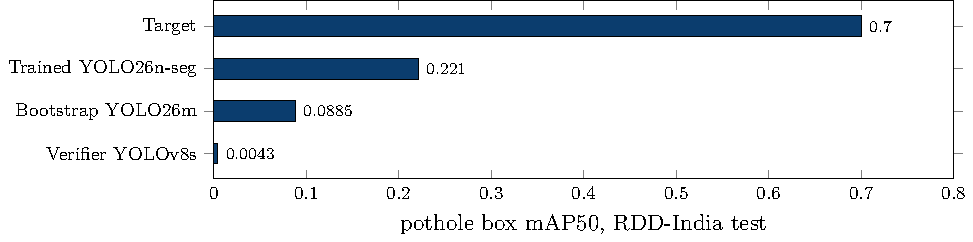
\includegraphics{figures/fig-10-ap-comparison.pdf}
\caption{The trained model is 2.5$\times$ the starter model, and about one third of the way to the 0.70 target.}
\end{figure}

\subsection{Per class (whole test split, 1,018 images)}
\begin{center}
\small
\begin{tabular}{@{}l r r r r r r@{}}
\toprule
\textbf{Class} & \textbf{GT objects} & \textbf{AP50} & \textbf{AP50-95} & \textbf{P@0.25} & \textbf{R@0.25} & \textbf{best F1}\\
\midrule
pothole & 1,038 & 0.217 & 0.072 & 0.502 & 0.127 & 0.303\\
alligator\_crack & 215 & 0.208 & 0.083 & 0.464 & 0.121 & 0.295\\
crack & 177 & 0.116 & 0.036 & 0.250 & 0.006 & 0.240\\
manhole & 69 & 0.099 & 0.062 & 0.157 & 0.159 & 0.179\\
\midrule
\textbf{mean (mAP)} & & \textbf{0.160} & \textbf{0.063} & & & \\
\bottomrule
\end{tabular}
\end{center}
For comparison, the verifier (YOLOv8s trained on all of RDD2022) is much better at cracks: alligator crack AP50 0.640
and crack 0.564. It therefore stays the verifier.

\subsection{Masks}
\begin{center}
\small
\begin{tabular}{@{}l r l@{}}
\toprule
\textbf{Mask metric (pothole)} & \textbf{Value} & \textbf{Note}\\
\midrule
Mask AP50 / AP50-95 & 0.228 / 0.081 & against SAM 2.1 pseudo-masks (test), at most 256\,px\\
Mean mask IoU of potholes found & \textbf{0.689} & over the 149 potholes found at confidence $\ge$ 0.25\\
Pixel IoU over all potholes & 0.266 & includes the missed ones\\
\bottomrule
\end{tabular}
\end{center}
\textbf{Reading this:} when the model finds a pothole, its outline overlaps the reference outline by about 69\,\% ---
good enough for area and volume. The problem is not the outline, it is that most potholes are not found.

\subsection{Against the acceptance targets (PLAN WP3)}
\begin{center}
\small
\begin{tabularx}{\textwidth}{@{}X r r c@{}}
\toprule
\textbf{Criterion} & \textbf{Target} & \textbf{Result} & \textbf{Status}\\
\midrule
Pothole box mAP50, RDD-India test & $\ge$ 0.70 (aim 0.75) & 0.221 & \fail\\
Box mAP50-95 & $\ge$ 0.45 & 0.072 & \fail\\
Mask IoU & $\ge$ 0.65 (aim 0.70) & 0.689 & \pass*\\
ONNX export within 2\,\% of the PyTorch mAP & --- & not done yet & \pending\\
\bottomrule
\end{tabularx}
\end{center}
*Only over the 149 potholes the model finds and against pseudo-masks; with a detector this weak it is not a strong
pass.

\subsection{What the predictions look like}
\begin{figure}[H]
\centering
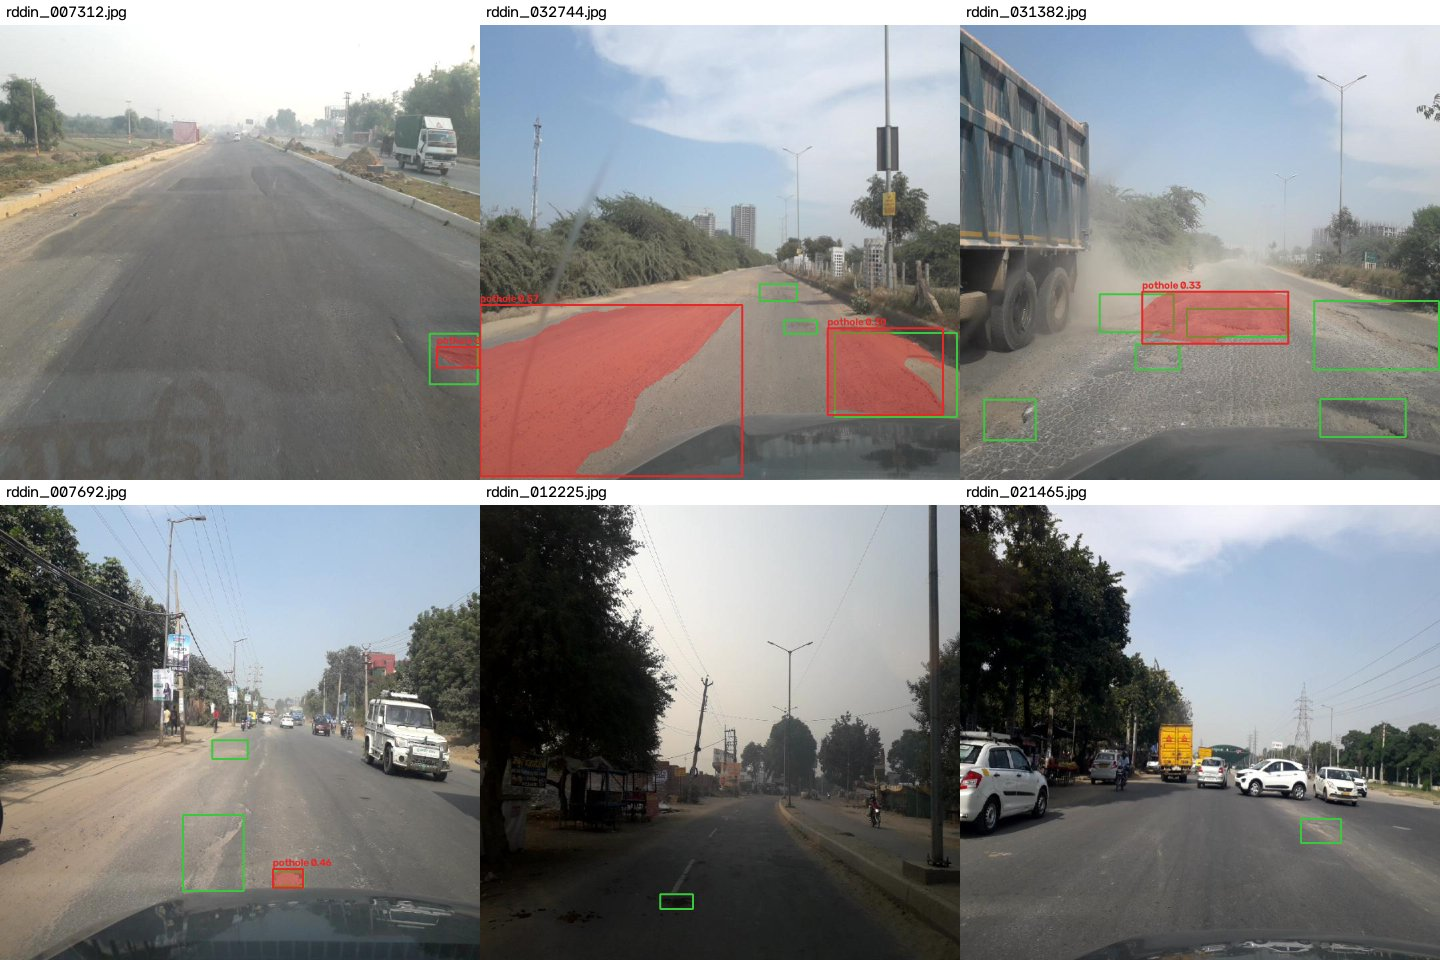
\includegraphics[width=\textwidth]{figures/predictions_rddin_test.jpg}
\caption{Trained model on RDD-India test images it never saw. \textcolor{gmok}{Green}: labelled potholes.
\textcolor{gmbad}{Red}: model output (mask, box, confidence) at confidence $\ge$ 0.25. Top row: correct finds
(left, right) and a large false positive on rough road (middle). Bottom row: a near miss next to a real pothole
(left) and small, distant potholes that are missed (middle, right). This is typical: big, close potholes are found;
small and distant ones are not.}
\end{figure}

\subsection{Why the score is low, and what will raise it}
\begin{center}
\small
\begin{tabularx}{\textwidth}{@{}>{\raggedright\arraybackslash}p{50mm} X@{}}
\toprule
\textbf{Cause} & \textbf{Remedy}\\
\midrule
Smallest model (3\,M parameters), 640\,px input: distant potholes are only a few pixels & YOLO26s-seg (11.5\,M) at 960\,px on the RTX 5080 (\code{make train PROFILE=rtx5080\_s})\\
Only 20 epochs, losses still falling & 80 epochs, mixed precision, larger batch on the RTX 5080\\
Recall 13\,\% at confidence 0.25; best F1 at confidence 0.08 & tune the confidence threshold in the pipeline; the verifier and multi-pass confirmation absorb extra false positives\\
Small, noisy validation set (174 potholes) & move part of the RDD-India pool into validation; pick the epoch by a smoothed score\\
Pseudo-masks and loose RDD boxes & 2\,\% human QC sample (\code{qc/label\_studio\_tasks.json}) and relabelling of the worst images\\
36\,\% non-Indian training frames & weigh Indian frames higher; add Telangana bus-camera frames from the pilot (pseudo-label, then review)\\
\bottomrule
\end{tabularx}
\end{center}

\subsection{How it is used meanwhile}
The trained model is now the system's segmenter (\code{SEG\_WEIGHTS} in \code{.env}; one line to switch back). It
beats the starter model on every pothole measure and is the first that gives outlines. A wrong detection does not go
straight into a work order: it must pass the verifier and be seen on $\ge$ 2 trips (Step 6) before it is confirmed.

% ================================================================================================ 10
\section{Measurement accuracy}\label{sec:measure}

\subsection{Geometry on exact synthetic data (verified)}
Rendered roads with a cavity of known shape, at known camera height and pitch. The depth map is exact, so this tests
the geometry and the $\sigma$ formulas, not a depth model.
\begin{center}
\footnotesize\setlength{\tabcolsep}{4pt}
\begin{tabular}{@{}l r r r r r@{}}
\toprule
\textbf{Case} & \textbf{True V, L} & \textbf{Meas.\ V, L} & \textbf{Err.} & \textbf{True p95} & \textbf{Meas.\ p95}\\
\midrule
car 1.4\,m, plane, cap 0.8\,m$\times$50\,mm @ 4\,m & 12.63 & $12.63\pm1.35$ & +0.0\,\% & 47.5 & 47.5\\
car 1.4\,m, plane, same cap @ 10\,m & 12.63 & $13.00\pm4.15$ & +2.9\,\% & 47.5 & 47.0\\
bus 2.4\,m, plane, same cap @ 5\,m & 12.63 & $12.63\pm2.77$ & +0.0\,\% & 47.5 & 47.5\\
bus 2.4\,m, crown, cap 1.0\,m$\times$70\,mm @ 8\,m & 27.72 & $27.69\pm6.77$ & $-0.1$\,\% & 66.8 & 66.7\\
car, plane, box 0.7\,m$\times$60\,mm @ 7\,m & 23.09 & $22.51\pm4.39$ & $-2.5$\,\% & 60.0 & 60.0\\
\bottomrule
\end{tabular}
\end{center}
All 16 cases pass (5 shown): maximum volume error 2.9\,\%, maximum p95 error 0.6\,mm. In 200 noisy trials the truth
was inside $\pm2\sigma$ every time (coverage 1.00 for depth, volume, area and width; target $\ge$ 0.90).

\subsection{Staged known-depth targets (rehearsed; real run pending)}
Foam-board ``potholes'' of 20/40/70\,mm filmed at 3--12\,m (\code{scripts/staged\_pothole\_truth.py}). Rehearsed on
rendered targets: depth error 1.7\,mm, volume error 12.0\,\%, IRC class 100\,\% (targets $\le$ 10\,mm, $\le$ 25\,\%,
$\ge$ 90\,\%). This tests the scripts, not a real camera.

\subsection{Real Indian road images (chain runs, not measurements)}
\begin{figure}[H]
\centering
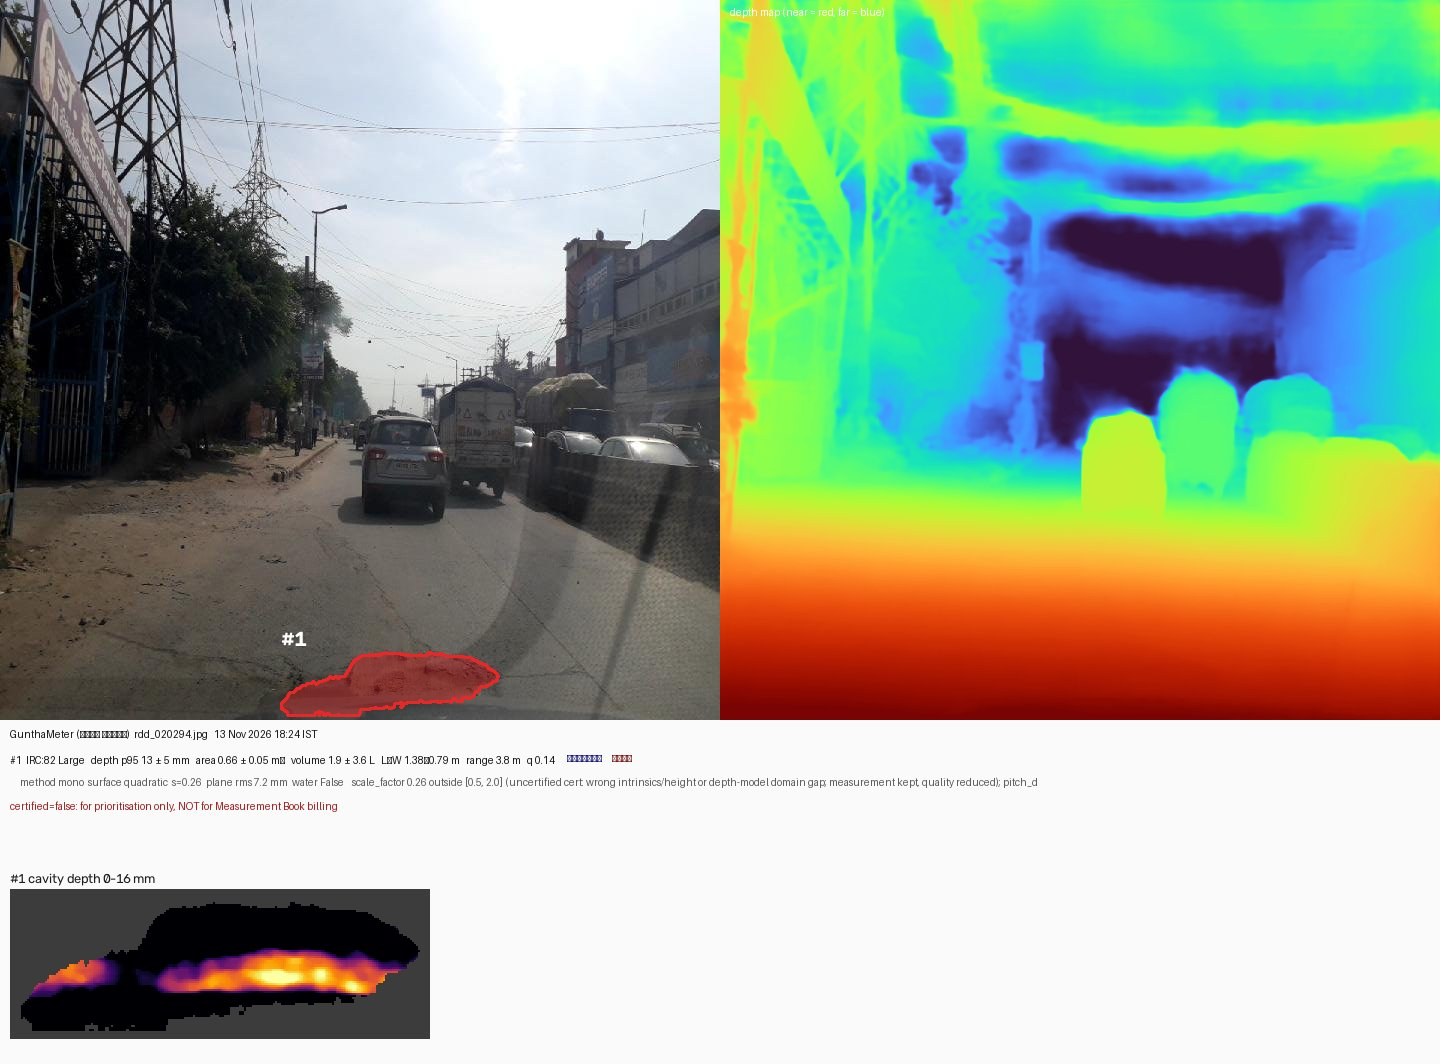
\includegraphics[width=0.92\textwidth]{figures/measure_overlay_rdd_020294.jpg}
\caption{The full measurement chain on a real RDD-India frame: pothole mask (left), metric depth map (right), cavity
depth (bottom). The camera height and angle of this photo are unknown, so the pipeline itself flags the result
(scale factor 0.26 outside 0.5--2.0, quality 0.14, \code{certified=false}). It demonstrates the chain and its safety
gates, not accuracy.}
\end{figure}

% ================================================================================================ 11
\section{The simulator and the end-to-end demo}\label{sec:demo}

Real buses are not yet equipped, so the loop is exercised with \emph{virtual buses} (\code{edge/sim/}): real TGSRTC
GTFS routes over real OpenStreetMap Hyderabad roads, real Indian pothole images pasted at geometrically correct
positions, GNSS noise and latency, the same protocol as a real device. Survey days, a repair day, verification days
and a DLP re-detection are scripted. \code{tasks.ps1 demo} runs it all from a clean database copy.

\begin{center}
\small
\begin{tabularx}{\textwidth}{@{}X r r@{}}
\toprule
\textbf{Demo run} (3 buses; routes 10H, 218, 5K; 2 days; 21 trips) & \textbf{Result} & \textbf{Target}\\
\midrule
Potholes confirmed & 43 & $\ge$ 30\\
Repairs verified by bus passes & 2 potholes / 3 work orders & $\ge$ 1\\
Reopened inside DLP, with a zero-pay rework order & 1 & $\ge$ 1\\
Jurisdiction-queue items & 4 & $\ge$ 1\\
Whole demo from a clean database copy & 732\,s & $<$ 20\,min\\
\midrule
Tomorrow's indent & \multicolumn{2}{r}{8 work orders, 49--60 bags (range), 3 circles}\\
30-day estimated repair cost vs baseline (2 zones) & \multicolumn{2}{r}{\INR63,922 vs \INR2,81,048}\\
\bottomrule
\end{tabularx}
\end{center}
In the demo the depth of each frame is a synthetic road render (method \code{synthetic}); the demo proves the pipeline
and operations loop, not measurement accuracy. It was last run with the starter detector (14 Nov).

% ================================================================================================ 12
\section{Size of the project}\label{sec:size}

\subsection{Code}
\begin{center}
\small
\begin{tabular}{@{}l r r l@{}}
\toprule
\textbf{Part} & \textbf{Files} & \textbf{Lines} & \textbf{Content}\\
\midrule
\code{server/} & 70 & 12,205 & API (55 endpoints), 34 database tables, workers, operations\\
\code{web/src/} & 55 & 6,855 & React PWA, Telugu/Hindi/English\\
\code{measure/} & 26 & 4,532 & depth, plane fit, cavity, $\sigma$, fusion, severity\\
\code{edge/} & 37 & 3,383 & simulator, protocol, Jetson stub, Android skeleton (Kotlin)\\
\code{geo/} & 21 & 3,220 & location, map-matching, clustering, passes\\
\code{ml/} & 10 & 2,916 & segmenter, training, evaluation, export\\
\code{tests/} & 25 & 2,618 & cross-module and end-to-end tests\\
\code{scripts/} & 15 & 2,535 & demo, validation, Windows tasks\\
\code{docs/} & 13 & 1,984 & plan, decisions, contracts, method, SOP, licences\\
\code{data/} (scripts) & --- & 1,962 & download, build, derive datasets\\
\code{repair/}, \code{priority/} & 18 & 2,086 & repair planner, priority and SLA\\
\code{gis/}, \code{configs/} & 24 & 984 & map layers, cameras, classes, profiles\\
\bottomrule
\end{tabular}
\end{center}
Lines count source, configuration and documentation in each folder (tests inside \code{server/}, \code{measure/} etc.\
are included there). By language, the repository holds 192 Python files with 34,452 lines and 53 TypeScript files with
6,772 lines. The GitHub repository (code, docs, configs, reports, no data or weights) is 416 files, 9.3\,MB.

\subsection{Tests}
276 Python tests (about 5--6 minutes), 38 web unit tests, 15 offline smoke checks and 3 browser end-to-end tests; the
code style checker (ruff) reports no issues.

\subsection{Data, models and outputs on disk}
\begin{center}
\small
\begin{tabular}{@{}l r@{}}
\toprule
\textbf{Item} & \textbf{Size}\\
\midrule
Original downloads (\code{data/raw}: RDD2022, eYantra, BharatPotHole, GTFS, OSM) & 13\,GB\\
Extracted data, SAM 2.1 mask cache, geo outputs (\code{data/interim}) & 3.4\,GB\\
Training datasets (\code{data/datasets}, both builds, hard-linked) & 788\,MB\\
Demo database (\code{data/gunthameter.db}, 454k road segments) & 131\,MB\\
Training run folder (21 checkpoints of 31.7\,MB + final weights) & 648\,MB\\
Model weights in \code{weights/} & 135\,MB\\
Hugging Face models (depth, SAM 2.1, SegFormer) & 577\,MB\\
\midrule
\textbf{Trained segmenter (\code{best.pt}) --- what a bus device needs} & \textbf{6.6\,MB}\\
\bottomrule
\end{tabular}
\end{center}

% ================================================================================================ 13
\section{Progress by work package}\label{sec:status}

\begin{longtable}{@{}p{0.29\textwidth} p{0.10\textwidth} p{0.55\textwidth}@{}}
\toprule
\textbf{Work package} & \textbf{State} & \textbf{Notes}\\
\midrule
\endhead
WP0 Scaffold and contracts & \done & frozen interfaces in \code{docs/CONTRACTS.md}\\
WP1 Data acquisition & \done & RDD2022, eYantra masks, SAM 2.1 pseudo-masks, 4-class dataset (6,416 images); OSM, GTFS\\
WP2 Measurement core & \done & synthetic 16/16, $\sigma$ coverage 1.00; real-camera accuracy pending\\
WP3 Training, export & \partly & code done; \textbf{first model trained} (box mAP50 0.221, target 0.70); RTX 5080 run and ONNX export pending\\
WP4 Database, API & \done & 55 endpoints, 34 tables, role-based access, audit log\\
WP5 Geo services & \done & PostGIS map-matching SQL never run against a real PostGIS\\
WP6 Workers & \done & nine pipeline stages, ops ticks, job poller\\
WP7 Edge simulator & \done & fleet acceptance 4/4; Android skeleton not compiled (no SDK); Jetson runner is a stub\\
WP8 Ops, repair planner & \done & state machines, SLA ladder, verification, DLP, runs, KPIs, MB/invoice exports\\
WP9 Web app & \done & tests, build, offline and browser tests pass; Lighthouse audit not run\\
WP10 GIS layers & \done & admin units are approximations marked \code{official: false}\\
WP11 Validation and docs & \done & method, calibration SOP, pilot plan, licences, demo script, report\\
WP12 End-to-end demo & \done & 732\,s from a clean copy; not yet run under Linux/WSL\\
\bottomrule
\end{longtable}

\begin{figure}[H]
\centering
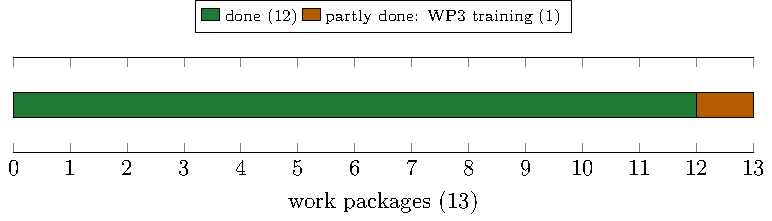
\includegraphics{figures/fig-11-wp-progress.pdf}
\end{figure}

% ================================================================================================ 14
\section{Pending steps}\label{sec:pending}

In the order they should be done. Durations are \emph{estimates} for one to two people.

\begin{longtable}{@{}p{0.03\textwidth} p{0.24\textwidth} p{0.48\textwidth} p{0.17\textwidth}@{}}
\toprule
\# & \textbf{Step} & \textbf{What has to happen} & \textbf{Estimate}\\
\midrule
\endhead
1 & Train a target-grade detector & YOLO26s-seg, 960\,px, 80 epochs on the RTX 5080 (\code{make train PROFILE=rtx5080\_s
NAME=y26s\_seg\_india}); evaluate; export to ONNX; tune the confidence threshold; regenerate the report. Target box
mAP50 $\ge$ 0.70. Data improvements of Section~\ref{sec:results} in parallel. & 1--2 weeks\\
2 & Licence decisions & Ultralytics AGPL (Enterprise licence, publish source, or RF-DETR); depth-model card; keep GPL-2
eYantra data out of a deployed model. & 1--2 weeks, in parallel\\
3 & Real-camera accuracy & Checkerboard calibration; film foam-board targets 20/40/70\,mm at 3--12\,m; run the
staged-truth script. Pass: depth error $\le$ 10\,mm, class accuracy $\ge$ 90\,\%, volume error $\le$ 25\,\%. & 2--4 weeks\\
4 & Android app & Android SDK build; on-device model (LiteRT); foreground service, IMU jolts, privacy blur, outbox. & 4--8 weeks\\
5 & Production set-up & PostgreSQL/PostGIS, object storage, GPU for depth, real secrets, demo mode off, backups,
security review, hosting in India. & 3--6 weeks, in parallel\\
6 & Smaller checks & Re-run the demo with the trained model; Lighthouse audit; fresh-eyes README run; Linux/WSL demo;
Telugu SOP review; official GHMC ward boundaries. & about 1 week\\
7 & Pilot & 20 buses at 3 depots; calibrate every bus; 2 weeks shadow mode, 10 weeks live through a monsoon; truth
campaign of 50--100 potholes per zone (\code{docs/DEPLOYMENT\_TSRTC.md}; indicative hardware \INR9--13 lakh). &
about 4 + 12 weeks\\
\bottomrule
\end{longtable}

\begin{figure}[H]
\centering
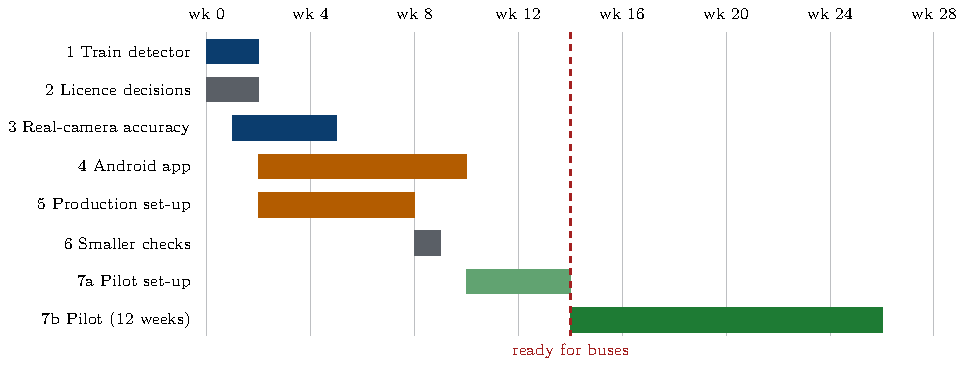
\includegraphics{figures/fig-12-timeline.pdf}
\caption{Indicative timeline (estimate): about 14 weeks to a bus-ready system; a validated pilot at about 26 weeks.}
\end{figure}

% ================================================================================================ 15
\section{How to run it}\label{sec:run}

On the Windows laptop, from \code{C:\textbackslash gunthameter} in PowerShell (Linux/WSL: \code{make <target>}):
\begin{center}
\small
\begin{tabularx}{\textwidth}{@{}l X@{}}
\toprule
\textbf{Command} & \textbf{What it does}\\
\midrule
\code{.\textbackslash scripts\textbackslash windows\textbackslash tasks.ps1 test} & all CPU tests (276, about 5--6 minutes)\\
\code{tasks.ps1 demo} & full end-to-end demo (API on port 8000, web on port 5173)\\
\code{tasks.ps1 measure-demo} & depth and volume on real Indian road images\\
\code{tasks.ps1 train} / \code{train-resume} & segmenter training in resumable 8-hour sessions\\
\code{tasks.ps1 eval --weights <best.pt> --stage <name>} & evaluate a model on the test split $\rightarrow$ \code{reports/model\_eval.json}\\
\code{tasks.ps1 report} & regenerate \code{reports/REPORT.md}\\
\bottomrule
\end{tabularx}
\end{center}
Demo logins (password \code{demo1234}): \code{admin}, \code{zonal\_khairatabad}, \code{engineer1}, \code{contractor1},
\code{contractor2}, \code{citizen1}. The active detector is set by \code{SEG\_WEIGHTS} in \code{.env}.

% ================================================================================================ A
\appendix
\section{Key documents and artefacts}
\begin{tabularx}{\textwidth}{@{}l X@{}}
\toprule
\code{docs/PLAN.md} & full design and work packages\\
\code{docs/DECISIONS.md} & deviations from the plan (D1--D15) and build status\\
\code{docs/HANDOFF.md} & where work stopped and next steps\\
\code{docs/CONTRACTS.md} & frozen interfaces, state machines, API list\\
\code{docs/DEPTH\_METHOD.md} & measurement method and validation\\
\code{docs/CALIBRATION\_SOP.md} & depot calibration (Telugu and English)\\
\code{docs/DEPLOYMENT\_TSRTC.md} & 20-bus pilot plan\\
\code{docs/LICENCES.md} & dataset, model and software licences\\
\code{data/datasets/india\_pothole\_seg4/stats.json} & dataset counts and the manhole re-split\\
\code{runs/seg/y26n\_seg\_india\_laptop/} & training run: settings, per-epoch log, checkpoints, \code{best.pt}\\
\code{reports/model\_eval.json} & every model evaluation\\
\code{reports/REPORT.md} & generated validation report\\
\bottomrule
\end{tabularx}

\section{Glossary}
\begin{tabularx}{\textwidth}{@{}l X@{}}
\toprule
$\sigma$ & standard uncertainty; the truth lies within $\pm2\sigma$ about 95\,\% of the time\\
$d_{p95}$ & 95th-percentile depth of the cavity, the design depth\\
IoU & intersection over union: overlap of two boxes or masks\\
AP, mAP & (mean) average precision: detector quality over all confidence thresholds\\
mAP50, mAP50-95 & mAP at IoU 0.5; averaged over IoU 0.5--0.95\\
Epoch & one pass of training over all training images\\
Pseudo-mask & a mask produced by a model (SAM 2.1) from a box, not drawn by a person\\
Transfer learning & starting training from a model already trained on other images\\
GFLOPs & billions of arithmetic operations per image (compute cost)\\
IRC & Indian Roads Congress (IRC:82, IRC:116, IRC:SP:100)\\
CRMP & Comprehensive Road Maintenance Programme (GHMC road packages)\\
DLP & defect-liability period\\
SLA & service-level agreement (repair deadline)\\
WO, MB & work order; Measurement Book (billing record)\\
GTFS, OSM & bus route and schedule format; OpenStreetMap\\
AE / DEE / EE & Assistant / Deputy Executive / Executive Engineer\\
PWA & progressive web app (installable, works offline)\\
\bottomrule
\end{tabularx}

\end{document}
